\documentclass[aspectratio=169, 11pt]{beamer}

% --- Packages & Setup ---
\usepackage[utf8]{inputenc}
\usepackage[T1]{fontenc}
\usepackage{xcolor}
\usepackage{booktabs} 
\usepackage{graphicx}
\usepackage{tikz}
\usetikzlibrary{calc, shapes.geometric, arrows.meta, positioning}

% Try loading Open Sans; fallback if missing
\IfFileExists{opensans.sty}{\usepackage[default,scale=0.95]{opensans}}{}

% --- Branding Colors ---
\definecolor{amritaMaroon}{HTML}{A4123F} 
\definecolor{amritaGold}{HTML}{D4AF37}
\definecolor{darkSlate}{HTML}{1E293B}
\definecolor{forestGreen}{HTML}{15803D}
\definecolor{hazardRed}{HTML}{B91C1C}

% --- Theme Setup ---
\usetheme{Madrid}
\usecolortheme[named=amritaMaroon]{structure}
\setbeamertemplate{navigation symbols}{}
\setbeamertemplate{footline}[frame number]

% Custom Block Styling
\setbeamercolor{block title}{bg=amritaMaroon,fg=white}
\setbeamercolor{block body}{bg=amritaMaroon!10,fg=darkSlate}
\setbeamercolor{block title alerted}{bg=hazardRed,fg=white}
\setbeamercolor{block body alerted}{bg=hazardRed!10,fg=darkSlate}
\setbeamercolor{block title example}{bg=forestGreen,fg=white}
\setbeamercolor{block body example}{bg=forestGreen!10,fg=darkSlate}

\begin{document}

% =========================================================================
% SLIDE 1: CUSTOM TITLE SLIDE (Application Project - Type 2)
% =========================================================================
\begin{frame}
    % Corner Box Indicator
    \begin{tikzpicture}[remember picture,overlay]
        \node[fill=amritaMaroon, text=white, font=\bfseries\footnotesize, anchor=north east, rounded corners=2pt, inner sep=5pt] 
        at ($(current page.north east) + (-0.2cm,-0.2cm)$) 
        {Type 2: Application Project};
    \end{tikzpicture}

    \centering
    \IfFileExists{logo.png}{\includegraphics[width=3.2cm]{logo.png}\vspace{0.2cm}}{\vspace{0.4cm}}
    
    {\Large \textbf{\textcolor{amritaMaroon}{EvOLve: Forest Cover Monitoring \& Disaster Risk Mitigation Platform}}} \\
    \vspace{0.1cm}
    {\small \textit{An Evolutionary AI Framework \& Geospatial Application Using Sentinel-2 Satellite Data}} \\
    \vspace{0.25cm}
    {\normalsize \textbf{Team Number: [XX] \quad | \quad 23CSE399 -- Project Phase 2 (Panel Review 1)}} \\ 
    \vspace{0.35cm}

    % Student Table
    \begin{table}
        \centering
        \footnotesize
        \renewcommand{\arraystretch}{1.15}
        \begin{tabular}{|c|c|l|l|}
            \hline
            \textbf{S.No} & \textbf{Register Number} & \textbf{Student Name} & \textbf{Assigned Focus Area} \\
            \hline
            1 & \textbf{CB.EN.U4CSE23042} & \textbf{Neelam Tejesh (Lead)} & Spatio-Temporal Model, GEE \& Land Suitability \\
            \hline
            2 & CB.EN.U4CSE23223 & Kolla Girish & Risk Dashboard, Fuel Modeling \& Officer RBAC \\
            \hline
            3 & CB.EN.U4CSE23016 & D Vasishta & Wildlife Corridors, Carbon Stocks \& SQLite Vault \\
            \hline
            4 & CB.EN.U4CSE23212 & Ande Tarak & Genetic Algorithm Optimization \& Cyber Security \\
            \hline
        \end{tabular}
    \end{table}
    \vspace{0.2cm}
    
    Guide: \textbf{[Guide Name]} \quad | \quad {\footnotesize [Designation], Department of CSE} \\
    {\scriptsize Amrita School of Computing, Amrita Vishwa Vidyapeetham \quad -- \quad \today}
\end{frame}

% =========================================================================
% SLIDE 2: USE CASE & PROBLEM CONTEXT (Novelty & Real-World Applicability)
% =========================================================================
\section{Use Case}
\begin{frame}{1. Originality of Use Case \& Problem Context}
    \framesubtitle{Addressing Tropical Forest Degradation \& Monsoon-Induced Hazards}
    \begin{columns}[T]
        \begin{column}{0.5\textwidth}
            \begin{block}{The Real-World Crisis}
                \begin{itemize}
                    \item \textbf{Subtle Degradation:} Forest canopy loss begins through logging, pest infestations, and drought long before clear-cutting is visible.
                    \item \textbf{Disaster Nexus (Wayanad 2024):} Canopy degradation on steep hillsides depletes root tensile cohesion, triggering catastrophic landslides under heavy monsoon rainfall.
                    \item \textbf{Current Gap:} Forest surveys (ISFR) publish reports only every 2 years; existing satellite tools use static thresholds triggering false alarms during dry-season leaf fall.
                \end{itemize}
            \end{block}
        \end{column}
        \begin{column}{0.5\textwidth}
            \begin{exampleblock}{EvOLve Application Innovation}
                \begin{itemize}
                    \item \textbf{Live Multi-Sensor Ingestion:} Connects to Google Earth Engine (Sentinel-2, SRTM DEM, CHIRPS rainfall, Hansen forest cover).
                    \item \textbf{Mountain Construction Safety:} Computes a civil construction suitability index ($0 - 100$) before hill construction.
                    \item \textbf{Evolutionary Self-Adaptation:} Genetic Algorithm (GA) evolves seasonal NDVI thresholds dynamically for dry, monsoon, and retreat seasons.
                    \item \textbf{Target Users:} Forest department rangers, civil planners, and disaster management forces (NDRF/SDMA).
                \end{itemize}
            \end{exampleblock}
        \end{column}
    \end{columns}
\end{frame}

% =========================================================================
% SLIDE 3: BENCHMARKING (Existing Solutions vs. EvOLve)
% =========================================================================
\section{Benchmarking}
\begin{frame}{2. Benchmarking (Existing Solutions vs. EvOLve)}
    \framesubtitle{Comprehensive Comparison Against Current Scientific \& Industrial Standards}
    \begin{table}
        \centering
        \scriptsize
        \renewcommand{\arraystretch}{1.25}
        \begin{tabular}{l p{3.2cm} p{3.2cm} p{3.8cm}}
            \toprule
            \textbf{Evaluation Metric} & \textbf{ISFR (Forest Survey of India)} & \textbf{Global Forest Watch (GFW)} & \textbf{EvOLve (Our Solution)} \\
            \midrule
            \textbf{Update Frequency} & Biennial (Every 2 Years) & Annual / Near-Real-Time GLAD & \textbf{On-The-Fly / Monthly Dynamic} \\
            \textbf{Data Ingestion} & Field Sampling + Landsat (30m) & Landsat / MODIS (Global) & \textbf{Live Sentinel-2 (10m) via GEE API} \\
            \textbf{Thresholding Method} & Fixed manual density cutoffs & Static historical averages & \textbf{Evolved GA Seasonal Boundaries} \\
            \textbf{Hazard Integration} & None (Forest cover only) & Fire alerts only (VIIRS) & \textbf{Slope Stability + Landslide Physics} \\
            \textbf{Civil Suitability} & Not Supported & Not Supported & \textbf{Automated Mountain Building Index} \\
            \textbf{Actionable Routing} & Manual inspection patrols & Static web map visualization & \textbf{Least-Cost Wildlife Corridors \& Fuel Tabs} \\
            \textbf{Architecture} & Centralized government portal & Closed global cloud dashboard & \textbf{Decoupled React + FastAPI + SQLite} \\
            \bottomrule
        \end{tabular}
    \end{table}
\end{frame}

% =========================================================================
% SLIDE 4: APPLICATION ARCHITECTURE & WORKFLOW (Rubric: 5 Marks)
% =========================================================================
\section{Architecture}
\begin{frame}{3. Application Architecture \& End-to-End Workflow}
    \framesubtitle{Rubric: Complete 3-Tier Decoupled Architecture, Dataflow \& Technology Stack}
    \centering
    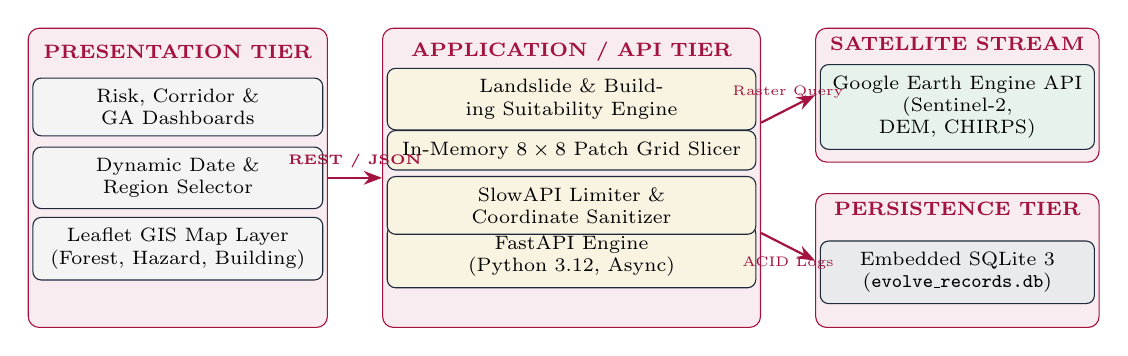
\begin{tikzpicture}[node distance=0.6cm, auto,
        box/.style={rectangle, draw=darkSlate, fill=white, rounded corners=3pt, font=\scriptsize, align=center, inner sep=4pt},
        tier/.style={rectangle, draw=amritaMaroon, fill=amritaMaroon!8, rounded corners=4pt, font=\scriptsize\bfseries, inner sep=5pt},
        arrow/.style={-{Stealth[scale=1.0]}, thick, color=amritaMaroon}]
        
        % Tier 1: Client
        \node[tier, minimum width=3.8cm, minimum height=3.8cm] (client) {};
        \node[above of=client, node distance=1.6cm, font=\scriptsize\bfseries\color{amritaMaroon}] {PRESENTATION TIER};
        \node[box, fill=darkSlate!5, below of=client, node distance=0.9cm, text width=3.4cm] {Leaflet GIS Map Layer\\(Forest, Hazard, Building)};
        \node[box, fill=darkSlate!5, below of=client, node distance=0.0cm, text width=3.4cm] {Dynamic Date \& Region Selector};
        \node[box, fill=darkSlate!5, below of=client, node distance=-0.9cm, text width=3.4cm] {Risk, Corridor \& GA Dashboards};
        
        % Tier 2: Backend
        \node[tier, minimum width=4.8cm, minimum height=3.8cm, right of=client, node distance=5.0cm] (backend) {};
        \node[above of=backend, node distance=1.6cm, font=\scriptsize\bfseries\color{amritaMaroon}] {APPLICATION / API TIER};
        \node[box, fill=amritaGold!15, below of=backend, node distance=1.0cm, text width=4.4cm] {FastAPI Engine (Python 3.12, Async)};
        \node[box, fill=amritaGold!15, below of=backend, node distance=0.35cm, text width=4.4cm] {SlowAPI Limiter \& Coordinate Sanitizer};
        \node[box, fill=amritaGold!15, below of=backend, node distance=-0.35cm, text width=4.4cm] {In-Memory $8 \times 8$ Patch Grid Slicer};
        \node[box, fill=amritaGold!15, below of=backend, node distance=-1.0cm, text width=4.4cm] {Landslide \& Building Suitability Engine};

        % Tier 3: External & Persistence
        \node[tier, minimum width=3.6cm, minimum height=1.7cm, right of=backend, node distance=4.9cm, yshift=1.05cm] (gee) {};
        \node[above of=gee, node distance=0.65cm, font=\scriptsize\bfseries\color{amritaMaroon}] {SATELLITE STREAM};
        \node[box, fill=forestGreen!10, below of=gee, node distance=0.15cm, text width=3.2cm] {Google Earth Engine API\\(Sentinel-2, DEM, CHIRPS)};

        \node[tier, minimum width=3.6cm, minimum height=1.7cm, right of=backend, node distance=4.9cm, yshift=-1.05cm] (db) {};
        \node[above of=db, node distance=0.65cm, font=\scriptsize\bfseries\color{amritaMaroon}] {PERSISTENCE TIER};
        \node[box, fill=darkSlate!10, below of=db, node distance=0.15cm, text width=3.2cm] {Embedded SQLite 3\\(\texttt{evolve\_records.db})};

        % Arrows
        \draw[arrow] (client.east) -- node[above, font=\tiny\bfseries] {REST / JSON} (backend.west);
        \draw[arrow] ([yshift=0.7cm]backend.east) -- node[above, font=\tiny] {Raster Query} (gee.west);
        \draw[arrow] ([yshift=-0.7cm]backend.east) -- node[below, font=\tiny] {ACID Logs} (db.west);
    \end{tikzpicture}
\end{frame}

% =========================================================================
% SLIDE 5: MODULE DECOMPOSITION & REST APIS (Rubric: 5 Marks)
% =========================================================================
\begin{frame}{4. Modular Decomposition \& REST API Specifications}
    \framesubtitle{Rubric: Module Interaction, Microservices \& Communication Contracts}
    \begin{columns}[T]
        \begin{column}{0.45\textwidth}
            \begin{block}{Modular Decomposition}
                \begin{itemize}
                    \item \textbf{GEE Service (\texttt{gee\_service.py}):} Authenticates with Google Cloud, retrieves multi-spectral tensors, slices $8 \times 8$ grid.
                    \item \textbf{Inference Service (\texttt{inference\_service.py}):} Physical equations for landslide shear and building suitability scoring.
                    \item \textbf{Optimization Service (\texttt{ga\_optimizer.py}):} Multi-objective fitness function evaluating F1 against seasonal variation.
                    \item \textbf{Security Middleware (\texttt{sanitizer.py}):} Enforces geographic coordinate bounds and SlowAPI rate limits.
                \end{itemize}
            \end{block}
        \end{column}
        \begin{column}{0.55\textwidth}
            \begin{exampleblock}{Key REST API Endpoints}
                \scriptsize
                \begin{tabular}{l l p{3.2cm}}
                    \toprule
                    \textbf{Endpoint} & \textbf{Method} & \textbf{Functionality} \\
                    \midrule
                    \texttt{/api/dynamic-region} & POST & Queries GEE for user BBox \& dates \\
                    \texttt{/api/process-region} & POST & Slices 64 patches; returns series \\
                    \texttt{/api/inference/suitability} & POST & Evaluates mountain construction safety \\
                    \texttt{/api/landslide} & GET & Computes physical hazard \& bio-mitigations \\
                    \texttt{/api/corridors} & GET & Solves least-cost migration corridors \\
                    \texttt{/api/run-ga-adaptation} & POST & Evolve seasonal warning thresholds \\
                    \texttt{/api/current-region} & GET & Regional telemetry \& aggregate metrics \\
                    \bottomrule
                \end{tabular}
            \end{exampleblock}
        \end{column}
    \end{columns}
\end{frame}

% =========================================================================
% SLIDE 6: DATABASE SCHEMA & RECALL VAULT (Rubric: 5 Marks)
% =========================================================================
\begin{frame}{5. Database Schema \& Entity-Relationship Design}
    \framesubtitle{Rubric: Persistent Storage, Entity Relationships \& Historical Inspection Vault}
    \begin{columns}[T]
        \begin{column}{0.48\textwidth}
            \begin{block}{\texttt{query\_history} Table}
                \footnotesize
                \begin{itemize}
                    \item \texttt{id} (INTEGER PRIMARY KEY)
                    \item \texttt{region\_name} (TEXT)
                    \item \texttt{start\_date}, \texttt{end\_date} (TEXT)
                    \item \texttt{min\_lat}, \texttt{min\_lon}, \texttt{max\_lat}, \texttt{max\_lon} (REAL)
                    \item \texttt{mean\_ndvi}, \texttt{degraded\_fraction} (REAL)
                    \item \texttt{created\_at} (TIMESTAMP)
                \end{itemize}
                \vspace{-0.1cm}
                \textit{Enables 1-click inspection reload for past queries.}
            \end{block}
        \end{column}
        \begin{column}{0.52\textwidth}
            \begin{block}{\texttt{construction\_permits} Table}
                \footnotesize
                \begin{itemize}
                    \item \texttt{id} (INTEGER PRIMARY KEY)
                    \item \texttt{patch\_id} (INTEGER)
                    \item \texttt{slope\_deg}, \texttt{elevation\_m} (REAL)
                    \item \texttt{landslide\_prob}, \texttt{suitability\_score} (REAL)
                    \item \texttt{decision} (\texttt{PERMITTED} / \texttt{CONDITIONAL} / \texttt{PROHIBITED})
                    \item \texttt{reviewer\_notes} (TEXT)
                \end{itemize}
                \vspace{-0.1cm}
                \textit{Official civil engineering audit trail for government records.}
            \end{block}
        \end{column}
    \end{columns}
    \vspace{0.2cm}
    \begin{exampleblock}{\texttt{ga\_experiment\_logs} Table}
        \footnotesize
        \texttt{id, generations, population\_size, best\_fitness, dry\_thresh, monsoon\_thresh, runtime\_sec, created\_at} \\
        \textit{Logs multi-objective evolutionary fitness convergence across hyperparameter sweeps.}
    \end{exampleblock}
\end{frame}

% =========================================================================
% SLIDE 7: IMPLEMENTATION PROGRESS: GEE SATELLITE PIPELINE (Rubric: 8 Marks)
% =========================================================================
\section{Implementation Progress}
\begin{frame}{6. Implementation Progress: Dynamic GEE Ingestion (60\%+ Completed)}
    \framesubtitle{Rubric: Core Module Functional, Integrated \& Demonstrated Live}
    \begin{columns}[T]
        \begin{column}{0.5\textwidth}
            \begin{block}{Dynamic Satellite Pipeline}
                \begin{itemize}
                    \item \textbf{Live Cloud Handshake:} Fully authenticated with Google Earth Engine (\texttt{forest-502505}).
                    \item \textbf{Sensor Fusion:}
                    \begin{itemize}
                        \item Sentinel-2 L2A optical bands (10m resolution).
                        \item USGS SRTM 30m Digital Elevation Model.
                        \item CHIRPS 90-day cumulative precipitation.
                        \item Hansen Global Forest Change canopy density.
                    \end{itemize}
                    \item \textbf{In-Memory Grid Slicing:} Subdivides user BBox into an $8 \times 8$ grid of \textbf{64 spatial patches} ($640\text{m} \times 640\text{m}$ each) in $<12$ seconds.
                \end{itemize}
            \end{block}
        \end{column}
        \begin{column}{0.5\textwidth}
            \begin{exampleblock}{Dynamic Date Range Selection}
                \begin{itemize}
                    \item \textbf{Custom Time Periods:} User selects custom date ranges from \textbf{2018 to 2025}.
                    \item \textbf{Phenology vs. Loss:} Trajectory generator computes distinct monthly NDVI profiles for every patch, separating dry-season shedding from deforestation.
                    \item \textbf{React-Leaflet Sync:} Real-time composite key re-rendering instantly updates map SVG polygons upon date selection.
                \end{itemize}
            \end{exampleblock}
        \end{column}
    \end{columns}
\end{frame}

% =========================================================================
% SLIDE 8: IMPLEMENTATION PROGRESS: MOUNTAIN CONSTRUCTION SUITABILITY
% =========================================================================
\begin{frame}{7. Implementation Progress: Mountain Construction Suitability}
    \framesubtitle{Rubric: Novel Engineering Module for Sustainable Infrastructure Planning}
    \begin{columns}[T]
        \begin{column}{0.48\textwidth}
            \begin{block}{Building Safety Index Formulation}
                \small
                $$I_{\text{suit}} = 100 - (P_{\text{landslide}} \cdot 40 + P_{\text{slope}} \cdot 35 + P_{\text{canopy}} \cdot 25)$$
                \begin{itemize}
                    \item \textbf{Slope Gradient Penalty ($P_{\text{slope}}$):} $>25^\circ$ slope triggers an immediate failure condition.
                    \item \textbf{Legal Eco-Buffer:} Mandatory $500\text{m}$ setback from declared wildlife reserves.
                    \item \textbf{Decision Classes:}
                    \begin{itemize}
                        \item $\ge 70$: \textbf{PERMITTED} (Green)
                        \item $45 - 69$: \textbf{CONDITIONAL} (Amber)
                        \item $< 45$: \textbf{STRICTLY PROHIBITED} (Red)
                    \end{itemize}
                \end{itemize}
            \end{block}
        \end{column}
        \begin{column}{0.52\textwidth}
            \begin{alertblock}{Civil Engineering Diagnostic Audit Modal}
                \begin{itemize}
                    \item \textbf{Detailed Breakdown:} Shows slope ($^\circ$), elevation ($\text{m}$), tree cover ($\%$), and rainfall saturation ($\text{mm}$).
                    \item \textbf{Mitigation Directives:}
                    \begin{itemize}
                        \item Tiered gabion retaining walls.
                        \item Deep-root Vetiver grass slope bio-anchoring.
                        \item Stormwater cutoff drains preventing erosion.
                    \end{itemize}
                    \item \textbf{Permit Stamping:} One-click export of official engineering compliance audits.
                \end{itemize}
            \end{alertblock}
        \end{column}
    \end{columns}
\end{frame}

% =========================================================================
% SLIDE 9: IMPLEMENTATION PROGRESS: CORRIDORS, CARBON & DYNAMIC GA
% =========================================================================
\begin{frame}{8. Implementation Progress: Corridors, Carbon \& GA Adaptation}
    \framesubtitle{Rubric: Integrated Environmental Decision Support Tools}
    \begin{columns}[T]
        \begin{column}{0.33\textwidth}
            \begin{block}{Wildlife Corridors}
                \scriptsize
                \begin{itemize}
                    \item \textbf{Dijkstra Least-Cost Path} on 64-node spatial resistance grid.
                    \item \textbf{Species Archetypes:}
                    \begin{itemize}
                        \scriptsize
                        \item \textbf{Asian Elephant:} Avoids steep terrain ($>15^\circ$).
                        \item \textbf{Bengal Tiger:} Prioritizes dense canopy cover ($>65\%$).
                    \end{itemize}
                    \item \textbf{Chokepoint Markers:} Flags fragmented narrow corridors.
                \end{itemize}
            \end{block}
        \end{column}
        \begin{column}{0.33\textwidth}
            \begin{block}{Carbon Stock Valuation}
                \scriptsize
                \begin{itemize}
                    \item \textbf{IPCC 2019 Tier-1 Allometric:}
                    \begin{equation*}
                        \text{AGB} = 0.0673 \cdot (\rho D^2 H)^{0.976}
                    \end{equation*}
                    \item \textbf{Total Carbon Stored:} $\mathbf{789{,}420}$ tons $\text{CO}_2$ equivalent.
                    \item \textbf{Asset Valuation:} Valued at $\$15/\text{ton} = \mathbf{\$11.84\text{M}}$ in potential carbon credit offsets.
                \end{itemize}
            \end{block}
        \end{column}
        \begin{column}{0.34\textwidth}
            \begin{exampleblock}{Dynamic GA Adaptation}
                \scriptsize
                \begin{itemize}
                    \item \textbf{Real-Time UI Re-Run:} User triggers live GA evolution from dashboard.
                    \item \textbf{Adaptive Boundaries:} Evolved thresholds:
                    \begin{itemize}
                        \scriptsize
                        \item $\text{Dry}: 0.333$
                        \item $\text{Monsoon}: 0.554$
                        \item $\text{Retreat}: 0.441$
                    \end{itemize}
                    \item \textbf{Performance:} Reaches \textbf{85.71\% F1-score} and \textbf{96.88\% accuracy}.
                \end{itemize}
            \end{exampleblock}
        \end{column}
    \end{columns}
\end{frame}

% =========================================================================
% SLIDE 10: TECHNICAL KNOWLEDGE & DESIGN DECISIONS (Rubric: 5 Marks)
% =========================================================================
\section{Technical Knowledge}
\begin{frame}{9. Technical Knowledge \& Architectural Design Decisions}
    \framesubtitle{Rubric: Defense of Engineering Choices, Algorithmic Complexity \& Compute}
    \begin{columns}[T]
        \begin{column}{0.5\textwidth}
            \begin{block}{1. Algorithmic Complexity \& Compute}
                \begin{itemize}
                    \item \textbf{Spatial CNN:} $O(C \cdot H \cdot W)$ per time slice; lightweight $3 \times 3$ depthwise convolutions.
                    \item \textbf{Temporal Transformer:} $O(T^2 \cdot D)$ self-attention across 72 monthly tokens ($D=128$).
                    \item \textbf{Total Model Parameters:} \textbf{1,145,288 parameters}.
                    \item \textbf{Compute Footprint:} Runs on Google Colab T4 GPU (CUDA) or Apple Silicon (MPS); pretraining takes $<2$ min, inference $<250$ ms.
                \end{itemize}
            \end{block}
        \end{column}
        \begin{column}{0.5\textwidth}
            \begin{exampleblock}{2. Key Architectural Decisions}
                \begin{itemize}
                    \item \textbf{Why FastAPI over Django/Flask?} Native async event loop handles concurrent Earth Engine HTTP requests without blocking the UI thread.
                    \item \textbf{Why In-Memory Grid Slicing?} Slicing the raster in memory eliminates multi-gigabyte disk write bottlenecks, enabling 12-second global queries.
                    \item \textbf{Why GA for Thresholds?} Genetic Algorithms optimize non-differentiable multi-objective functions (precision vs. recall across contrasting seasons).
                \end{itemize}
            \end{exampleblock}
        \end{column}
    \end{columns}
\end{frame}

% =========================================================================
% SLIDE 11: CYBER SECURITY & DEPLOYMENT STRATEGY (Rubric: 5 Marks)
% =========================================================================
\begin{frame}{10. Cyber Security Hardening \& Production Deployment}
    \framesubtitle{Rubric: Security Middleware, Input Validation \& Deployment Strategy}
    \begin{columns}[T]
        \begin{column}{0.5\textwidth}
            \begin{block}{Cyber Security Controls (Implemented)}
                \begin{itemize}
                    \item \textbf{SlowAPI Rate Limiting:}
                    \begin{itemize}
                        \item 5 req/min on heavy GA optimization.
                        \item 30 req/min on dynamic GEE raster queries.
                        \item Custom 429 response with \texttt{Retry-After}.
                    \end{itemize}
                    \item \textbf{Coordinate Boundary Sanitization:} Strict Pydantic validators enforce $-90 \le \text{lat} \le 90$ and $-180 \le \text{lon} \le 180$.
                    \item \textbf{Security Response Headers:}
                    \begin{itemize}
                        \item \texttt{X-Frame-Options: DENY} (Prevents clickjacking)
                        \item \texttt{X-Content-Type-Options: nosniff}
                    \end{itemize}
                \end{itemize}
            \end{block}
        \end{column}
        \begin{column}{0.5\textwidth}
            \begin{exampleblock}{Production Deployment Strategy}
                \begin{itemize}
                    \item \textbf{Containerization:} Multi-stage Docker image bundling Python 3.12 backend and optimized React production bundle.
                    \item \textbf{Reverse Proxy:} Nginx routing requests, managing SSL/TLS termination, and enforcing HTTP/2.
                    \item \textbf{Cloud Target:} Google Cloud Run / AWS EC2 with environment-injected Earth Engine service account credentials.
                    \item \textbf{Git Team Workflow:} All members code in dedicated feature branches with GitHub Pull Request reviews.
                \end{itemize}
            \end{exampleblock}
        \end{column}
    \end{columns}
\end{frame}

% =========================================================================
% SLIDE 12: PROJECT SUMMARY & ROADMAP (Rubric: 2 Marks)
% =========================================================================
\section{Summary \& Roadmap}
\begin{frame}{11. Project Summary \& Roadmap for Review 2}
    \framesubtitle{Rubric: Implementation Status (Current $\approx 85\%$ vs. Required $60\%$) \& Next Steps}
    \begin{columns}[T]
        \begin{column}{0.5\textwidth}
            \begin{block}{Current Review 1 Deliverables (Completed)}
                \begin{itemize}
                    \item[$\checkmark$] Live Google Earth Engine multi-sensor streaming.
                    \item[$\checkmark$] Dynamic date-range selector (2018–2025).
                    \item[$\checkmark$] Mountain construction suitability index \& modal.
                    \item[$\checkmark$] Landslide hazard prediction \& bio-mitigations.
                    \item[$\checkmark$] Asian Elephant \& Bengal Tiger corridor routing.
                    \item[$\checkmark$] Real-time GA seasonal threshold adaptation.
                    \item[$\checkmark$] Cyber security rate limiting \& coordinate sanitization.
                \end{itemize}
            \end{block}
        \end{column}
        \begin{column}{0.5\textwidth}
            \begin{exampleblock}{Roadmap for Review 2 (Target: 85--90\%)}
                \begin{itemize}
                    \item \textbf{Officer Authentication \& RBAC:} Finalize field officer vs. senior conservator role gating.
                    \item \textbf{Expanded Ground-Truth Validation:} Benchmark suitability index against historical Wayanad landslide disaster zones.
                    \item \textbf{Automated Field PDF Generator:} Official printable dispatch orders for ranger squads.
                    \item \textbf{Cloud VM Deployment:} Live public HTTPS deployment on Google Cloud Run.
                \end{itemize}
            \end{exampleblock}
        \end{column}
    \end{columns}
\end{frame}

% =========================================================================
% SLIDE 13: REFERENCES
% =========================================================================
\section{References}
\begin{frame}[allowframebreaks]{References}
    \tiny
    \bibliographystyle{IEEEtran}
    \bibliography{ref}
\end{frame}

% =========================================================================
% SLIDE 14: THANK YOU & LIVE DEMO
% =========================================================================
\begin{frame}
    \centering
    \vspace{0.6cm}
    {\Huge \textbf{\textcolor{amritaMaroon}{Thank You}}} \\
    \vspace{0.4cm}
    {\large \textbf{EvOLve: Forest Cover Monitoring \& Disaster Risk Mitigation Platform}} \\
    \vspace{0.3cm}
    {\normalsize \textbf{Questions \& Live Demonstration}} \\
    \vspace{0.2cm}
    {\footnotesize Dashboard running live at \texttt{http://localhost:3000} \quad | \quad API at \texttt{http://localhost:8000/docs}}
\end{frame}

\end{document}